\documentclass[11pt]{article}

% Change "review" to "final" to generate the final (sometimes called camera-ready) version.
% Change to "preprint" to generate a non-anonymous version with page numbers.
\usepackage[review]{acl}

% Standard package includes
\usepackage{times}
\usepackage{latexsym}
\usepackage{amsmath}
\usepackage{booktabs}
\usepackage{tabularx}

% For proper rendering and hyphenation of words containing Latin characters (including in bib files)
\usepackage[T1]{fontenc}

% This assumes your files are encoded as UTF8
\usepackage[utf8]{inputenc}

% This is not strictly necessary, and may be commented out,
% but it will improve the layout of the manuscript,
% and will typically save some space.
\usepackage{microtype}

% This is also not strictly necessary, and may be commented out.
% However, it will improve the aesthetics of text in
% the typewriter font.
% \usepackage{inconsolata}

% Including images in your LaTeX document requires adding
% additional package(s)
\usepackage{graphicx}
\usepackage{xcolor}

\newcommand{\am}[1]{\textcolor{orange}{[AM: #1]}}
\newcommand{\jb}[1]{\textcolor{blue}{[JB: #1]}}

% If the title and author information does not fit in the area allocated, uncomment the following
%
%\setlength\titlebox{<dim>}
%
% and set <dim> to something 5cm or larger.

\title{Read, Translate, Write: LLMs Translate with Fuzzy Semantic Hubs}

% Author information can be set in various styles:
% For several authors from the same institution:
% \author{Author 1 \and ... \and Author n \\
%         Address line \\ ... \\ Address line}
% if the names do not fit well on one line use
%         Author 1 \\ {\bf Author 2} \\ ... \\ {\bf Author n} \\
% For authors from different institutions:
% \author{Author 1 \\ Address line \\  ... \\ Address line
%         \And  ... \And
%         Author n \\ Address line \\ ... \\ Address line}
% To start a separate ``row'' of authors use \AND, as in
% \author{Author 1 \\ Address line \\  ... \\ Address line
%         \AND
%         Author 2 \\ Address line \\ ... \\ Address line \And
%         Author 3 \\ Address line \\ ... \\ Address line}

\author{First Author \\
  Affiliation / Address line 1 \\
  Affiliation / Address line 2 \\
  Affiliation / Address line 3 \\
  \texttt{email@domain} \\\And
  Second Author \\
  Affiliation / Address line 1 \\
  Affiliation / Address line 2 \\
  Affiliation / Address line 3 \\
  \texttt{email@domain} \\}

\begin{document}
\maketitle
\begin{abstract}

\end{abstract}

\section{Introduction}

Machine translation has long been an influential area of natural language processing. The attention mechanism was first proposed to improve machine translation performance \citep{bahdanau2015neuralmachinetranslationjointly,luong-etal-2015-effective,vaswani2017attention}; one consequence of attention was the emergence of language models that could be efficiently trained on massive corpora \citep{devlin-etal-2019-bert,radford2018improving}. So-called large language models (LLMs) have revolutionized many areas of natural language processing, but have been relatively slowly adopted in machine translation (MT).

A reason for the slow adoption of LLMs in MT has been a focus on low-resource languages, where LLMs face significant challenges \citep{hendy2023goodgptmodelsmachine,robinson2023chatgptmtcompetitivehigh}. Because LLMs require large training corpora, they are difficult to train effectively on low-resource languages. However, they also hold significant promise: even when not trained on a given language, LLMs can be prompted to translate from or into a language they have seen very little of in their training data \citep{cahyawijaya-etal-2024-llms}---e.g., by prompting with a grammar book \citep{tanzer2024a}. Moreover, their representations of high-resource languages could enable cross-lingual transfer \citep{conneau-etal-2020-unsupervised} with little data in the target language.

Whether LLMs can deliver on this promise depends in part on the mechanisms underlying how they translate. Specifically, do LLMs rely on task- and language-agnostic mechanisms to translate, or are they more specialized to specific language pairs? If the former, this opens up a clear path toward improving MT performance, potentially without large parallel corpora \citep{artetxe2018unsupervised}. Much recent work provides mechanistic evidence supporting this hypothesis in the language modeling context \citep{wendler-etal-2024-llamas,brinkmann-etal-2025-large,wu2025the}. We therefore posit that LLMs might translate using the same mechanisms they use to language model: the ``stages of inference'' hypothesis  \citep{lad2024the} holds that LLMs devote the first half of their layers to reading an input and composing increasingly abstract concept representations . Then, the latter half of the model reads these concept representations, and uses them to decide which token should be predicted given prior context. This implies that translation would not necessarily require language pair--specific mechanisms: instead, it only requires that a model be capable of reading abstract features from the source language, and generating text for the target language conditioned on those features.
% This means that the middle layers of a model are essentially ``semantic hubs'' \aaron{cite} containing a few concepts that explain much of the variance in the pretraining corpus.

If this hypothesis is true, it has three main implications for MT. (1) Given language pair $(S,T)$, translation performance should be predictable from monolingual capabilities in $S$ and $T$ in isolation without cross-linguistic interaction terms. (2) There should exist task-agnostic representations that are causally relevant for predicting correct outputs in both machine translation \emph{and} monolingual language modeling settings. Finally, (3) adding translation capabilities for a new language should only require improvements to monolingual capabilities for that language---i.e., monolingual corpora should yield similar improvements in translation performance as parallel corpora, assuming the model can already effectively handle the other language in the language pair.

We investigate each of these three implications, and find positive evidence for each. While no single experiment is a smoking gun confirming the noisy channel hypothesis, each provides convergent evidence in support of it. This could provide a preliminary explanation for the value of exposure to (largely monolingual) documents in producing models more effective at translation.

\section{Related Work}
\paragraph{Massively multilingual feature representations.} Our work is partially motivated by the observation that grammatical concept representations are highly multilingual in large language models, even across typologically distinct language pairs \citep{brinkmann-etal-2025-large}. Similar evidence has been observed in \citep{wendler-etal-2024-llamas,dumas-etal-2025-separating}.

\paragraph{Interpretability.}

\paragraph{Low-resource machine translation.} 

\section{A Motivating Observation: Monolingual Capabilities Explain Translation Performance}
How much of a model's ability to translate can be explained by its monolingual language modeling capabilities? We start by defining a \textbf{linear model} from monolingual competence to translation competence.

We use accuracies on MultiBLiMP as a proxy for monolingual competence. We take the macroaverage of scores across BLiMP categories for a given language.

For translation, we have language pair $(S, T)$, where $S$ is the source and $T$ is the target language. Translation competence $t_{ST}$ is quantified as a BLEU score for $(S, T)$. For each language pair, we measure $l_S$ and $l_T$, and learn coefficients $\beta_S$ and $\beta_T$ to maximize predictive accuracy in the following function:
\begin{equation}
    \beta_S l_S + \beta_Tl_T = t_{ST}
\end{equation}
We hypothesize that if a model is encoding an input into some universal feature space, then the predictive power of this model will be high. If a model relies on specialized translation mechanisms, the predictive power should be relatively low.

For further context, we also train a bilinear model with an interaction term:
\begin{equation}
    \beta_Sl_S + \beta_Tl_T + \beta_{ST}l_{ST} = t_{ST}
\end{equation}
If our hypothesis is correct, then the bilinear model should not have significantly greater predictive power than the linear model.

\am{TODO: results}

\am{TODO @Jake: slot in the BLiMP vs.\ BLEU figures from `v2.tex`}

\begin{figure}[t]
\centering
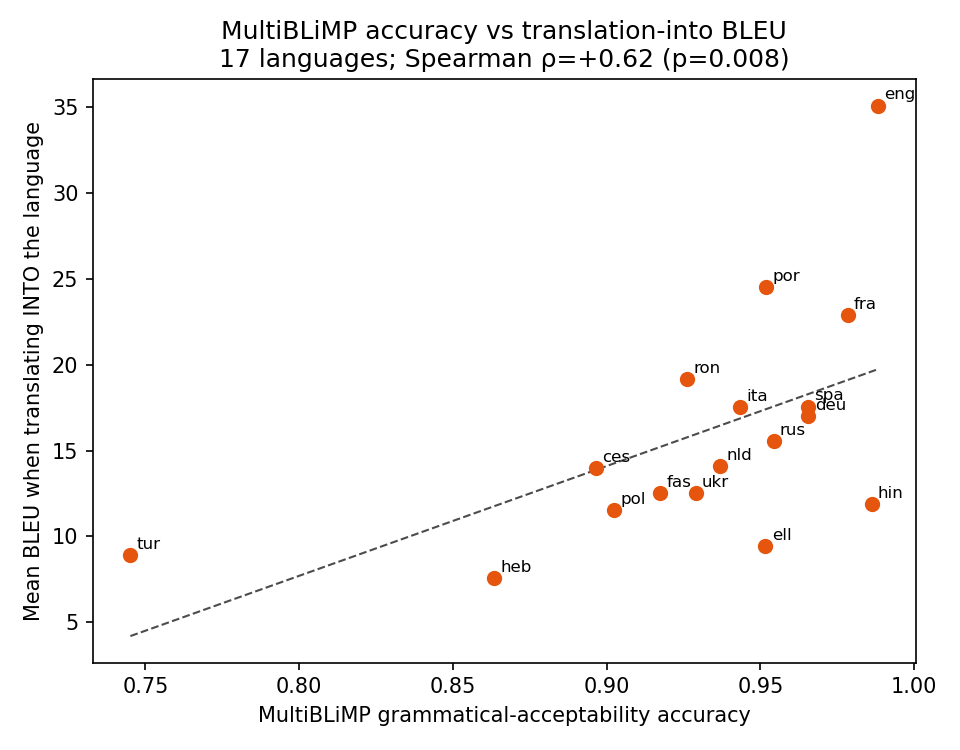
\includegraphics[width=.82\linewidth]{figures/fig_multiblimp_marginal.png}
\caption{MultiBLiMP minimal pair accuracy vs. mean BLEU when translating into each language, over 17 Multi-BLiMP languages \jb{According to Claude, (\texttt{ces, deu, ell, eng, fas, fra, heb, hin, ita, nld, pol, por, ron, rus, spa, tur, ukr}). TODO: verify}. Spearman $\rho=+0.62$ ($p=0.008$).}
\label{fig:proxy}
\end{figure}

\begin{figure}[t]
\centering
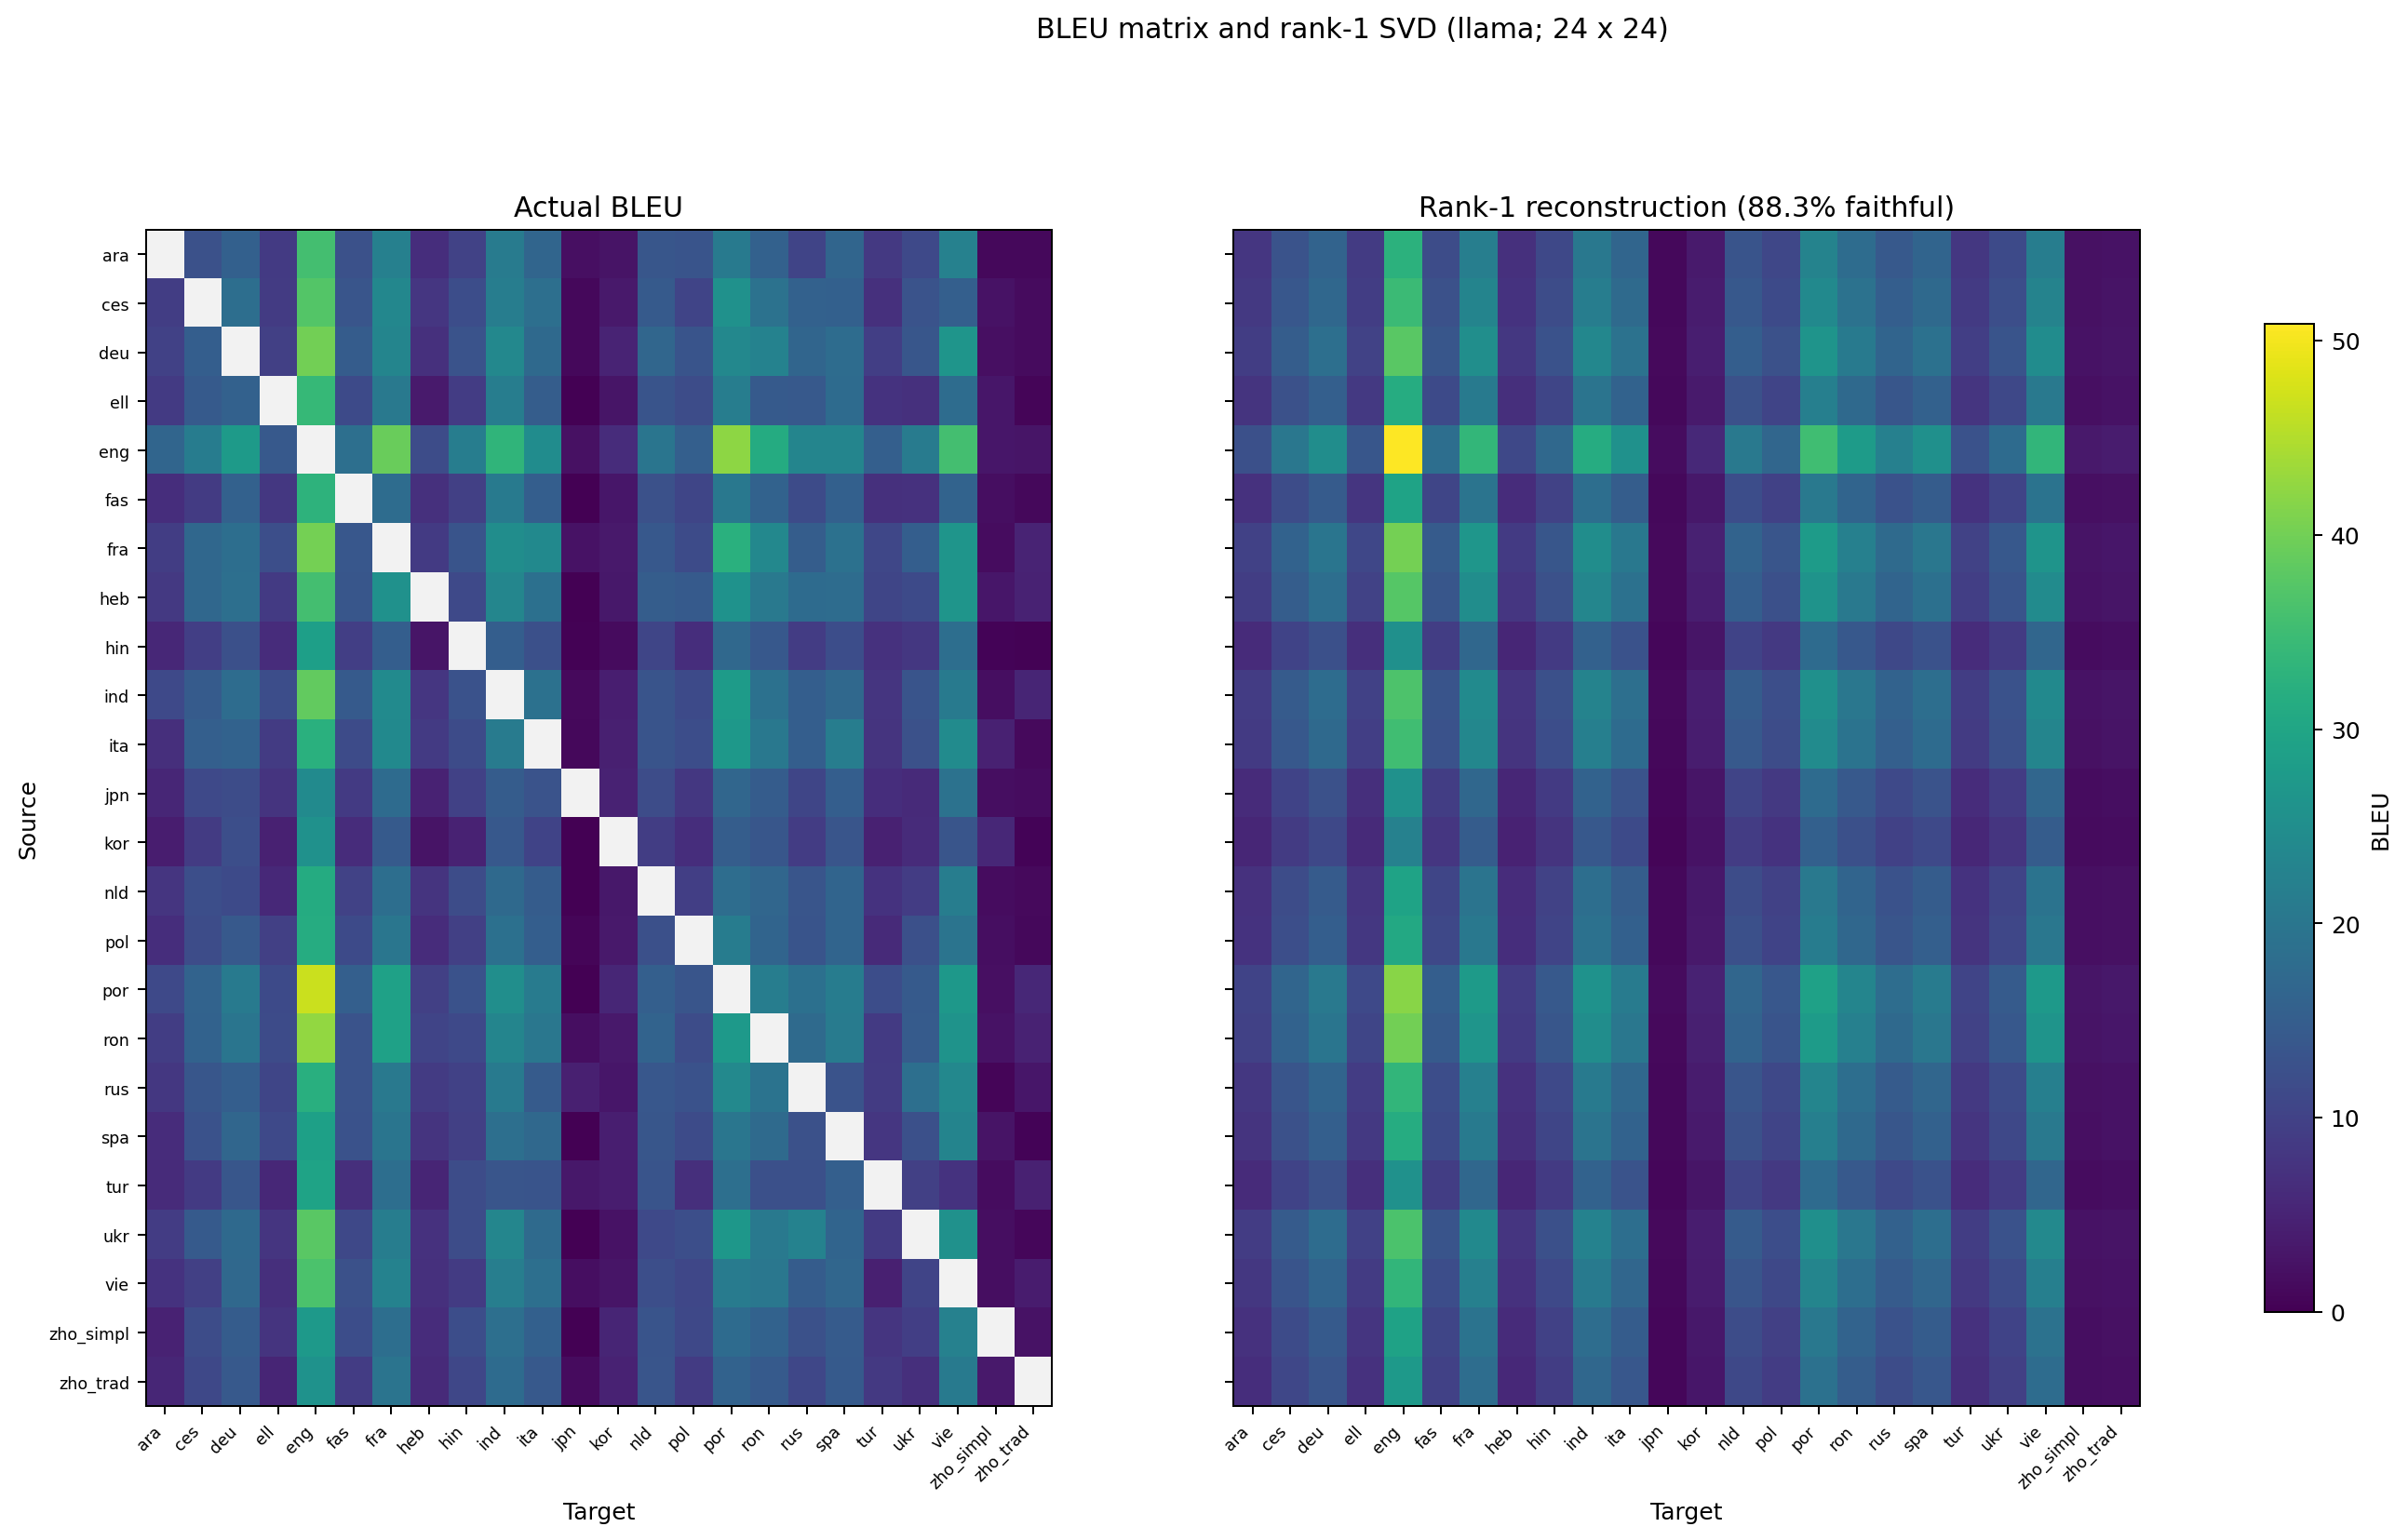
\includegraphics[width=\linewidth]{figures/bleu_matrix_rank1_llama.png}
\caption{Llama BLEU matrix and its rank-1 SVD reconstruction. The missing cells along the diagonal are imputed by the mean of the target column. \jb{TODO: mask the diagonal out instead of imputation, I think this would overestimate the faithfulness}}
\label{fig:rank1}
\end{figure}
% \jb{Comment from an audit: Mean-imputation can inflate the low-rank fit; a masked / observed-cells-only recompute is the clean check (PAPER\_TODO A1).}}

% \section{Ablations of attention heads that distinguish valid translations from random sentences}

% Quick explanation of GCM

% Identification of top heads via GCM (i.e. the heads with the largest indirect effect)

% Then we investigate what ablating these heads does on BLiMP minimal pairs

% $\Delta$ is the difference between 


\section{Many Translation-Relevant Components Perform Monolingual Language Modeling}

We turn our attention to show, mechanistically, that the model components implicated in translation are oftentimes those responsible for core language modeling in the monolingual setting.

\subsection{Using GCM to Identify Translation-relevant Components}

We search for model components that are causal in promoting the valid translation over an invalid, but grammatically correct counterfactual.

Set $(p_{\text{orig}}, r_{\text{orig}}, r_{\text{cf}})$ where $p_{\text{orig}}$ is the prompt with two candidate continuations $r$ and define this preference metric:
\begin{equation}
M = \log \pi(r_{\text{cf}}\mid p_{\text{orig}}) - \log \pi(r_{\text{orig}}\mid p_{\text{orig}}),
\label{eq:metric}
\end{equation}
where $\log\pi(r\mid p) = \sum_t \log p(r_t \mid p, r_{<t})$ is the
teacher-forced log-probability of a continuation, summed over its tokens. $M$ is thus the model's log-odds preference for $r_{\text{cf}}$ over $r_{\text{orig}}$ under the same prompt. We then take a model component as a mediator; call its activation $z$. Then $M(z)$ becomes the above metric as a function of $z$ when all other components are held constant. The change in $M$ when moving from the counterfactual to the original \jb{Is this correct? I'm thinking about pos/neg here} is the indirect effect:

\begin{equation}
\mathrm{IE}_{\text{patch}}(z) = M(z_{\text{orig}}) - M(z_{\text{cf}}).
\label{eq:patch}
\end{equation}

\jb{The following a summary from Claude, do we keep something like this or refer to the paper?}
\paragraph{The GCM estimator.} GCM \citep{sankaranarayanan2026gcm} removes the
per-component cost by linearizing $M$ around $z_{\text{orig}}$. A first-order
Taylor expansion gives $M(z_{\text{cf}}) \approx M(z_{\text{orig}}) + \nabla_z
M|_{z_{\text{orig}}}\!\cdot(z_{\text{cf}} - z_{\text{orig}})$; substituting into
Eq.~\ref{eq:patch},
\begin{equation}
\widehat{\mathrm{IE}}(z) = \nabla_z M\big|_{z=z_{\text{orig}}} \cdot (z_{\text{orig}} - z_{\text{cf}}).
\label{eq:ie}
\end{equation}
This recovers $\mathrm{IE}_{\text{patch}}$ to first order but is computable for
\emph{every} component at once: the gradients $\nabla_z M$ come from a single
backward pass, and the deltas $(z_{\text{orig}} - z_{\text{cf}})$ from caching
each component's activation on the original and counterfactual runs. So one
forward$+$backward pass yields an IE estimate for all $1024$ heads and all
$32{,}768$ SAE features, versus one patched forward pass \emph{each} for the
exact version.

The magnitude of the indirect effect is how much of the model's preference flows through this component when all else is kept constant. Because we define $M = m_{\text{cf}} - m_{\text{orig}}$, components with a positive indirect effect push the model towards $r_\text{cf}$, and those with a negative indirect effect push the model towards $r_\text{orig}$. \jb{Maybe this is flipped?}

Now, we can set $r_{\text{orig}}$ to be a gold translation of the original source, and $r_{\text{cf}}$ a grammatically correct but invalid translation. We do this using the FLORES parallel corpus \jb{TODO: cite}. Given a source and target language, we construct a prompt as follows:

\jb{From Claude:}
% ===================== OPTION A: real FLORES sentences (English -> Spanish) =====================
The two shots are a fixed, held-out pair of FLORES sentences (rows 0--1, the same
two for every direction); separators are single newlines and the final line ends
in a trailing space, so the response begins as a bare target token:
\begin{quote}\ttfamily\small\setlength{\parindent}{0pt}
English: On Monday, scientists from the Stanford University School of Medicine announced the invention of a new diagnostic tool that can sort cells by type: a tiny printable chip that can be manufactured using standard inkjet printers for possibly about one U.S. cent each.\\
Spanish: El lunes, los científicos de la facultad de medicina de la Universidad de Stanford anunciaron el invento de una nueva herramienta de diagnóstico que puede catalogar las células según su tipo: un pequeñísimo chip que se puede imprimir y fabricar con impresoras de inyección de uso corriente, por un posible costo de, aproximadamente, un centavo de dólar por cada uno.\\
English: Lead researchers say this may bring early detection of cancer, tuberculosis, HIV and malaria to patients in low-income countries, where the survival rates for illnesses such as breast cancer can be half those of richer countries.\\
Spanish: Los principales investigadores principales sostienen que esto puede permitir la detección precoz del cáncer, la tuberculosis, el VIH y la malaria en pacientes de países de bajos recursos, donde la tasa de supervivencia de enfermedades como el cáncer de mama puede ser la mitad de la de los países más avanzados.\\
English: The JAS 39C Gripen crashed onto a runway at around 9:30 am local time (0230 UTC) and exploded, closing the airport to commercial flights.\\
Spanish:
\end{quote}
Under this single prompt we score two candidate continuations: the gold target
$r_{\text{orig}} =$ ``\texttt{El JAS 39C Gripen impactó contra una pista cerca de
las 9:30 de la mañana hora local (0230 UTC) y explotó, lo que causó el cierre del
aeropuerto para vuelos comerciales.}'' and a counterfactual $r_{\text{cf}} =$ the
gold translation of a different source, ``\texttt{Se identificó al piloto como
Dilokrit Pattavee, líder de escuadrón.}'' (grammatical Spanish, but not a valid
translation of the query).

% ===================== OPTION B: schematic template =====================
The two shots are a fixed, held-out pair of FLORES sentences (the same two for
every language direction); separators are single newlines and the final line
ends in a trailing space, so the response begins as a bare target token:
\begin{quote}\ttfamily
[source language]: (source sentence 1)\\
{}[target language]: (target sentence 1)\\
{}[source language]: (source sentence 2)\\
{}[target language]: (target sentence 2)\\
{}[source language]: (query source sentence)\\
{}[target language]:
\end{quote}
where \texttt{[source language]} / \texttt{[target language]} are the language
names (e.g.\ English / Spanish), the first two pairs are held-out FLORES sentence
pairs, and under this single prompt we score two continuations: the gold target
$r_{\text{orig}}$ (the true translation of the query) and a counterfactual
$r_{\text{cf}}$ (the gold target of a \emph{different} source --- grammatical but
not a valid translation of the query).
\jb{End Clauding}

We patch at the last source token position only. For each of the 56 ordered cross-language pairs in \{English, Spanish, German, French, Turkish, Arabic, Hindi, Hebrew\}, we compute the IE for attention heads and SAE features.

However, this process could be simply isolating components that distinguish between the content of $r_{\text{orig}}$ and $r_{\text{cf}}$. As control tasks, we modulate over two factors, where ``Cross---Real'' is the original experiment:
\begin{itemize}
    \item Linguality:
    \begin{itemize}
        \item ``Same'' refers to when $S=T$
        \item ``Cross'' is when translation is performed (i.e. the languages are distinct)
    \end{itemize}
    \item Validity: 
    \begin{itemize}
        \item ``Real'' indicates that we have chosen the valid translation as $r_{\text{orig}}$
        \item ``Null'' is when both $r_{\text{orig}}$ and $r_{\text{cf}}$ are random samples
    \end{itemize}
\end{itemize}

\jb{TODO: decide on a format for real/null same/cross}

In particular, $\textsc{real\_cross}-\textsc{null\_cross}$ measures whether the component is in a translation-specific circuit or merely a multilingual one. $\textsc{null\_same}$ measures the pure content discrimination floor.

\jb{Here, I do think that the attention heads are not as discriminative as we've hoped, as $\textsc{real\_cross}-\textsc{null\_cross}$ is not that large of a difference for most heads. It does seem like SAE features do have a cleaner separation.}

\begin{figure}[t]
\centering
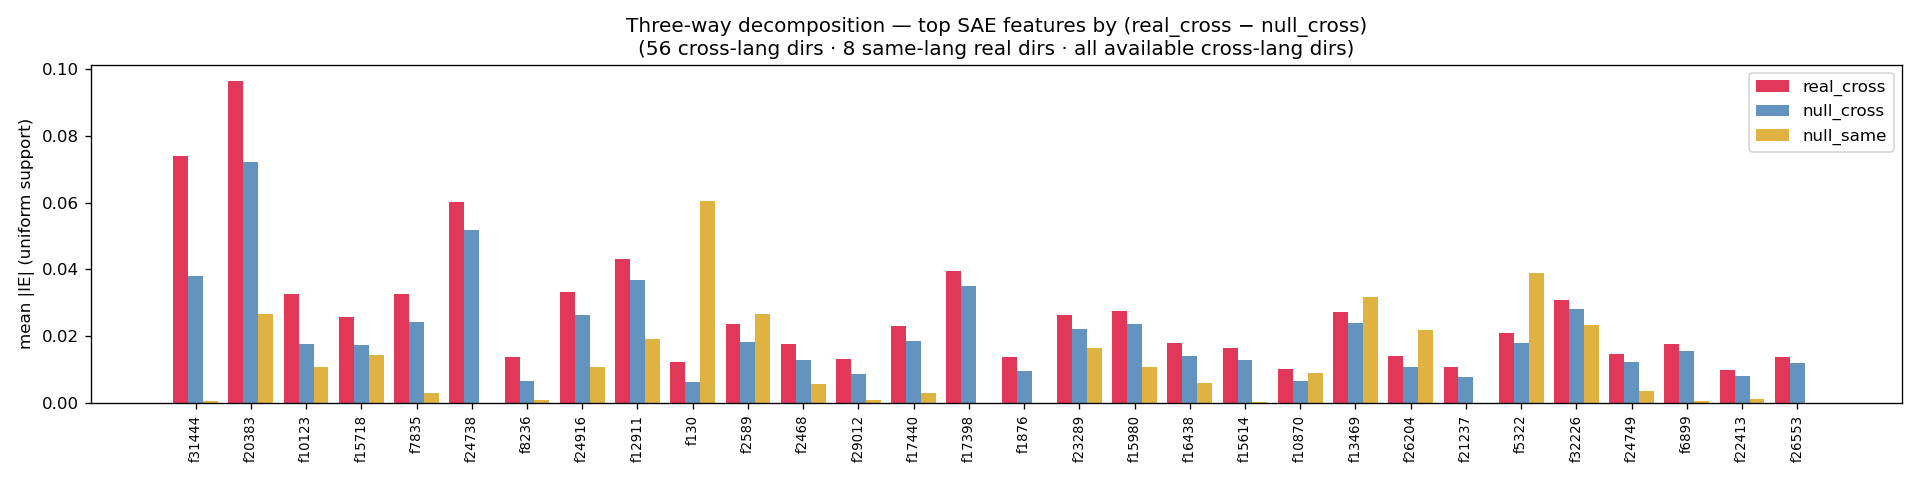
\includegraphics[width=\linewidth]{figures/three_way_decomposition_sae_full.png}
\caption{Comparison of GCM results and control tasks. These are the top SAE features as sorted by $\textsc{real\_cross} - \textsc{null\_cross}$. The bars represent the mean $|\widehat{\mathrm{IE}}|$ of \textsc{real\_cross}, \textsc{null\_cross}, and \textsc{null\_same}.}
\label{fig:gcm-decomp}
\end{figure}

\begin{figure}[t]
\centering
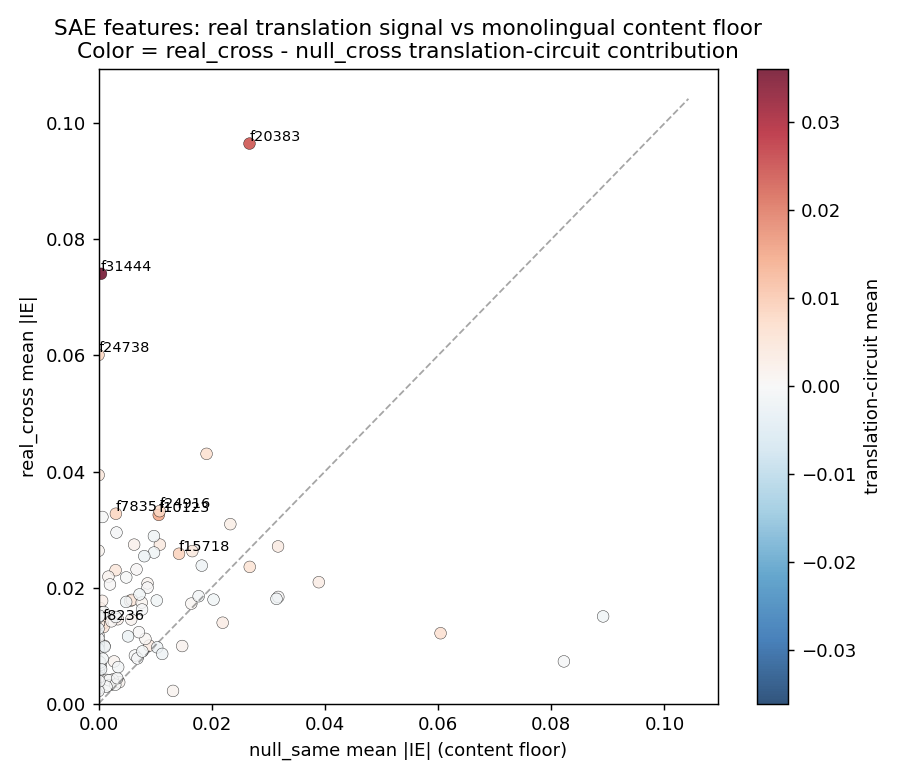
\includegraphics[width=\linewidth]{figures/meeting_sae_real_vs_null_same.png}
\caption{Here is the (\textsc{real\_cross}) mean
$|\widehat{\mathrm{IE}}|$ plotted against the content-discrimination floor
(\textsc{null\_same}). Features well above the diagonal are active in translation contexts but not as much in monolingual settings. One such example is f31444, which had the largest absolute difference between \textsc{real\_cross} and \textsc{null\_cross}.}
\label{fig:gcm-sae-realnull}
\jb{Maybe it would be better to swap out null\_same for null\_cross and just have the plot be of that, with no color? OR swap for real\_same, but real\_same is kinda measuring copying a little bit instead of monolingual as we'd like it to}
\end{figure}

\subsection{Signedness of Indirect Effect of Heads Predicts Monolingual Grammatical Performance}

We have found some model components responsible for differentiating between correct and incorrect translations. Is it possible that these same components are responsible for core language modeling?

\jb{On second thought, we should be trying some control task here where we ablate heads that were found in the null GCM experiments (i.e. still had high IE just not for translation)}

We use the Multi-BLiMP dataset, which contains minimal pairs of grammatical concepts, which measure the model's ability to perform agreement tasks matching the subject to some target which must match in Person, Number, or Gender. We measure the model's ability to distinguish between correct and incorrect completions. We take a random 400 (200 for Hebrew and Hindi) examples, resulting in a mix of tasks. An example:

\jb{TODO: This table is from Claude, so will need to verify that this is in fact an actual example, plus clean up the width}
\begin{table}[t]
\centering
\small
\setlength{\tabcolsep}{3pt}
\renewcommand{\arraystretch}{1.08}
\begin{tabularx}{\linewidth}{@{}l X l l@{}}
\toprule
Lang / phenomenon & Prefix & Gram. & Ungram. \\
\midrule
eng SV-P (Person 3$\to$1) &
\texttt{For one thing, there} &
\texttt{is} &
\texttt{am} \\

eng SV-\# (Number Sg$\to$Pl) &
\texttt{The below site from the US government} &
\texttt{verifies} &
\texttt{verify} \\

fra SV-P (Person 1$\to$3) &
\texttt{Oui, madame Schroedter, j'} &
\texttt{examinerai} &
\texttt{examinera} \\

fra SP-G (Gender M$\to$F) &
\texttt{Combien de temps a} &
\texttt{duré} &
\texttt{durée} \\
\bottomrule
\end{tabularx}
\caption{Representative MultiBLiMP minimal pairs. $\Delta>0$ when the model prefers the grammatical continuation.}
\label{tab:multiblimp-examples}
\end{table}

For each target language $L$ in the GCM languages, we aggreate the GCM head indirect effects over the 7 directions where $L$ is a distinct language. This allows us to select the top 20 heads by the mean $|\widehat{IE}|$, splitting the heads into POS and NEG categories based on their sign. Each Multi-BLiMP minimal pair is scored by the following:

\begin{equation}
\Delta = \log p(\texttt{correct completion} | \texttt{prefix}) \\ - \log p(\texttt{incorrect completion} | \texttt{prefix})
\end{equation}

Now, we can compute the \emph{difference in deltas} between the ablated and original models. That is, $\Delta_{change} = \Delta_{ablation} - \Delta_{original}$. The ablated model is produced by ablating the top 20 heads to their mean output at that position. A negative $\Delta_{change}$ means that the ablation weakened the model's ability to distinguish between the correct and incorrect completions, the expected behavior.

\begin{figure}[t]
\centering
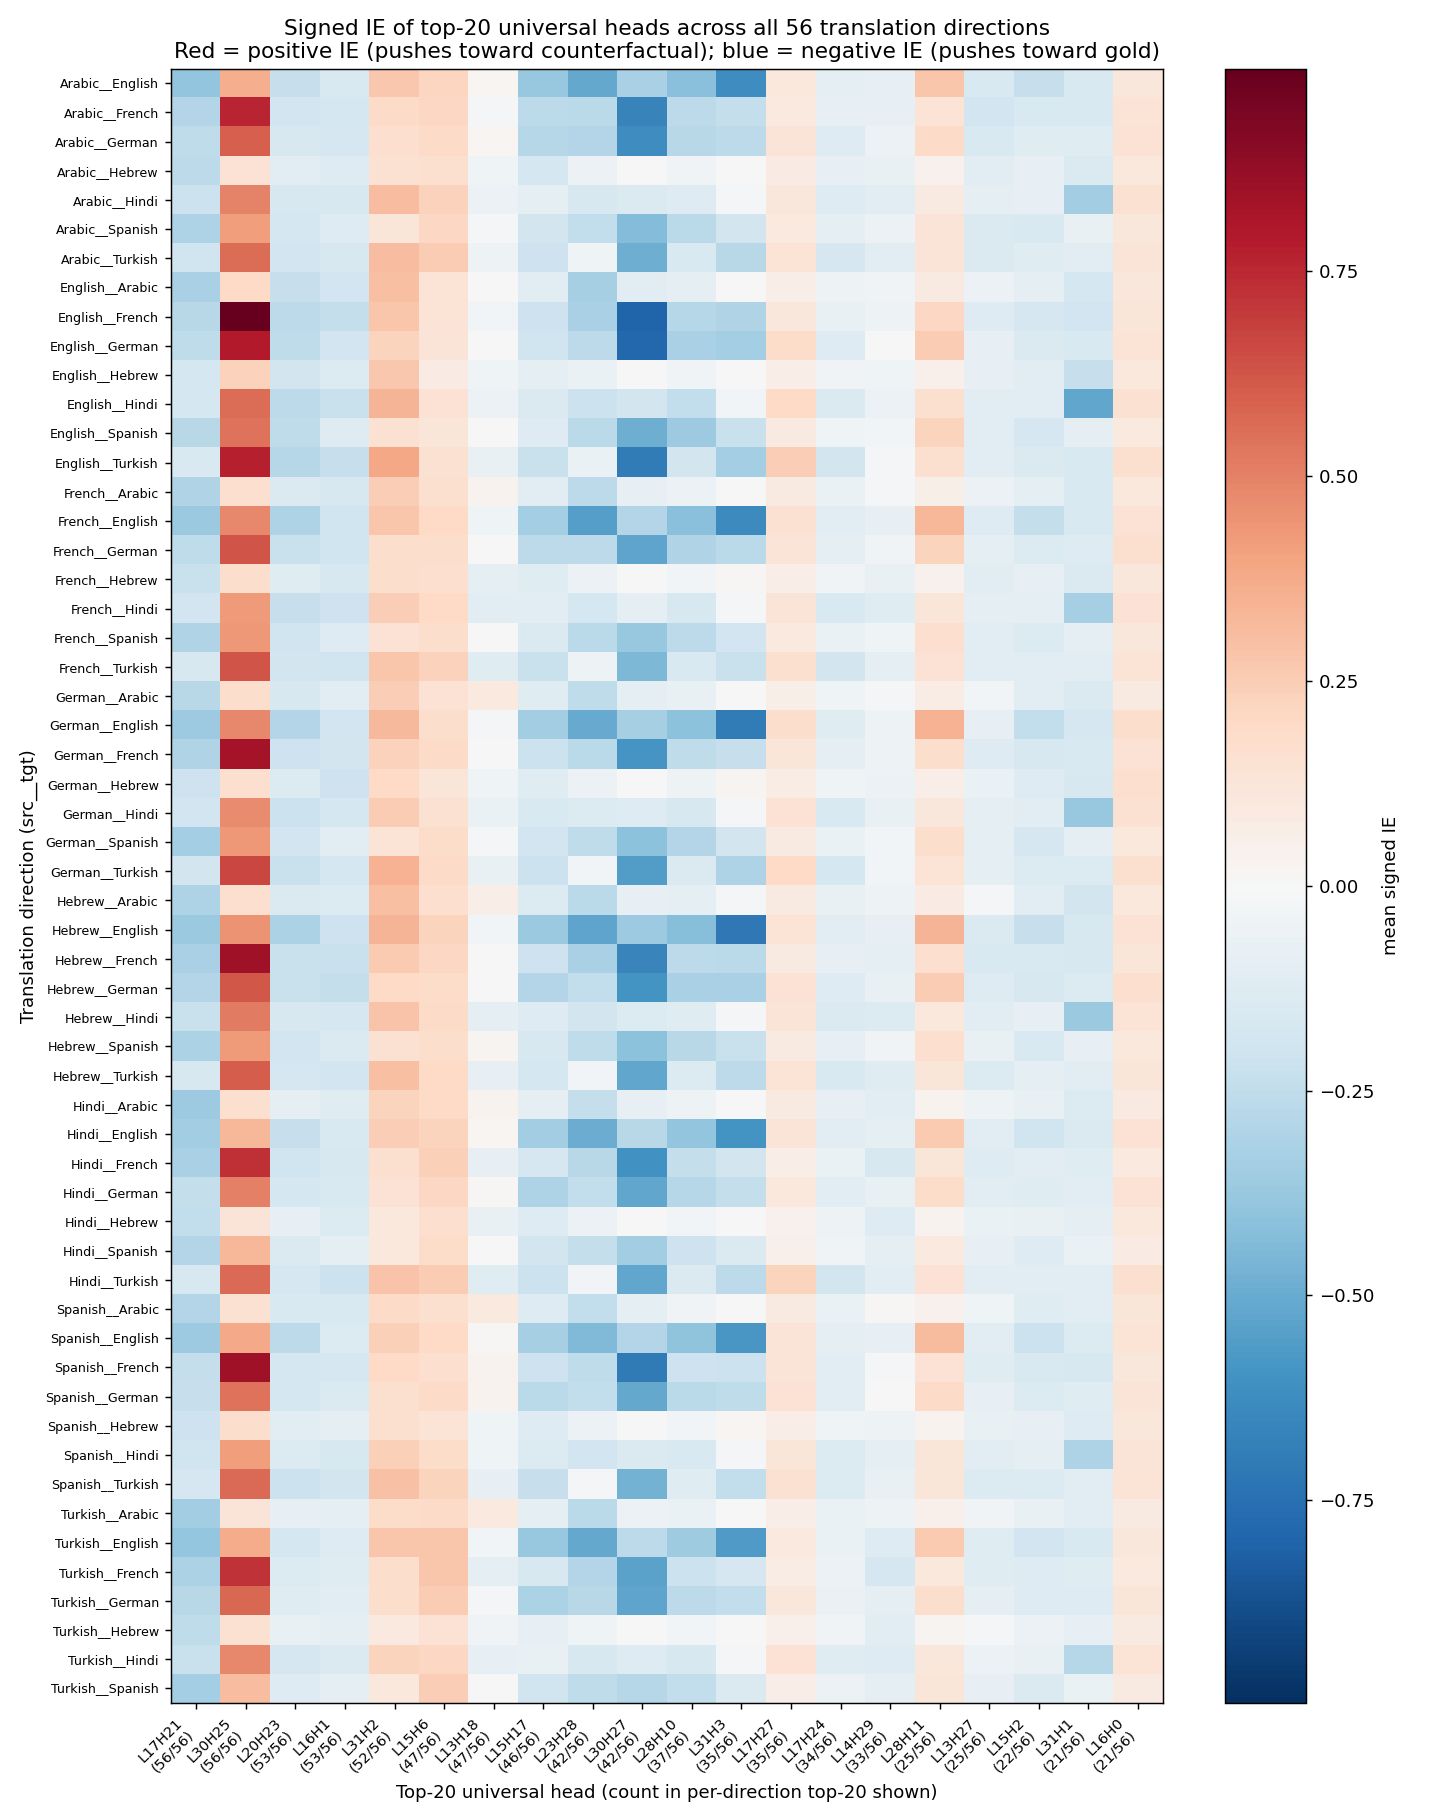
\includegraphics[width=\linewidth]{figures/meeting_direction_by_universal_head_signed.png}
\caption{Signed IE of the top-$20$ universal heads across all $56$
cross-language directions. Red cells indicate positive IE (the head's original state pushes toward the counterfactual response); blue cells indicate negative IE (pushes toward the gold response). The x-axis is sorted from left to right by the number of directions of which the head has a top 20 indirect effect.}
\label{fig:gcm-signed-heads}
\end{figure}


\begin{figure}[t]
\centering
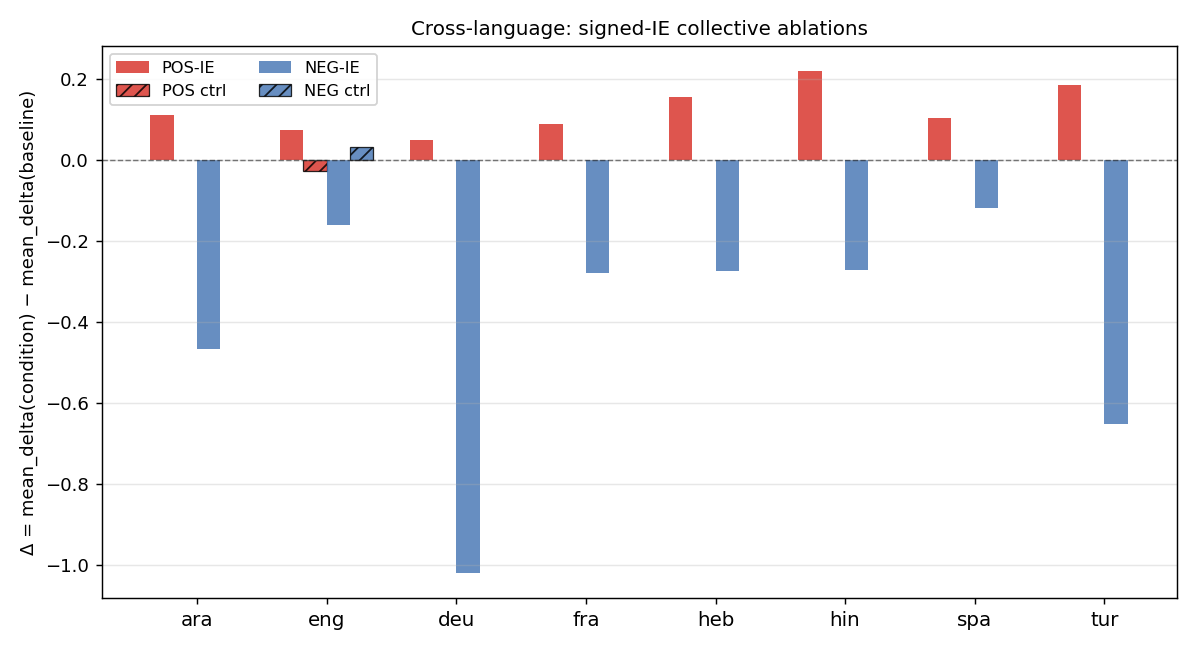
\includegraphics[width=\linewidth]{figures/cross_lang_sign_split.png}
\caption{Per-language $\Delta_{\text{change}}$ on Multi-BLiMP from ablating the
\textsc{pos}-signed vs.\ \textsc{neg}-signed sub-population of the top-$20$ GCM
heads. Negative means ablation weakened the grammaticality preference. Produced
by \texttt{visualize.py} from \texttt{analysis\_summary.csv}.}
\jb{TODO: run the control ablations for non-English langs}
\label{fig:ablate-signsplit}
\end{figure}


\jb{TODO: write the results paragraph for this. As a placeholder, here's something that Claude came up with:}
\paragraph{Result: GCM sign predicts the monolingual ablation effect.} In all
eight languages, ablating the \textsc{neg}-signed sub-population
\emph{weakened} the grammaticality margin ($\Delta_{\text{change}}$ from $-0.12$
to $-1.02$), while ablating the \textsc{pos}-signed sub-population
\emph{strengthened} it ($+0.05$ to $+0.22$). A property measured purely in the
translation task---the sign of a head's GCM indirect effect---thus predicts the
direction of its causal effect on a monolingual grammaticality task. The
\textsc{neg}-signed heads (the majority, $\sim$65--80\% of the top-$20$) behave
like shared language-modeling machinery that translation borrows; the smaller
\textsc{pos}-signed population behaves like translation-specific routing, whose
removal does not carry monolingual grammaticality information. By contrast, the
mixed top-$5$ collective and the random controls are at the noise floor in
$7/8$ languages, because a set chosen by absolute IE alone mixes the two
opposing populations. For the one language with size-matched controls so far
(English---the only completed $53$-condition v2 run), the matched-size POS/NEG
random controls sit near zero ($-0.028$, $+0.032$) while the sign-split groups
are several times larger ($+0.075$, $-0.160$), an early sign that the effect is
not a group-size artifact; matched controls for the other seven languages are
queued (job \texttt{5772145}, n=400, A100).
\jb{End Claude}

\subsection{Grammatically-derived Features}

\jb{This section is sparse because I'm not sure if we'd keep it. But we could give an account of how we derived the grammatical concepts SAE features (input and output) from UD, then show that there is some overlap between those SAE features and the GCM SAE features}
\begin{figure}[t]
\centering
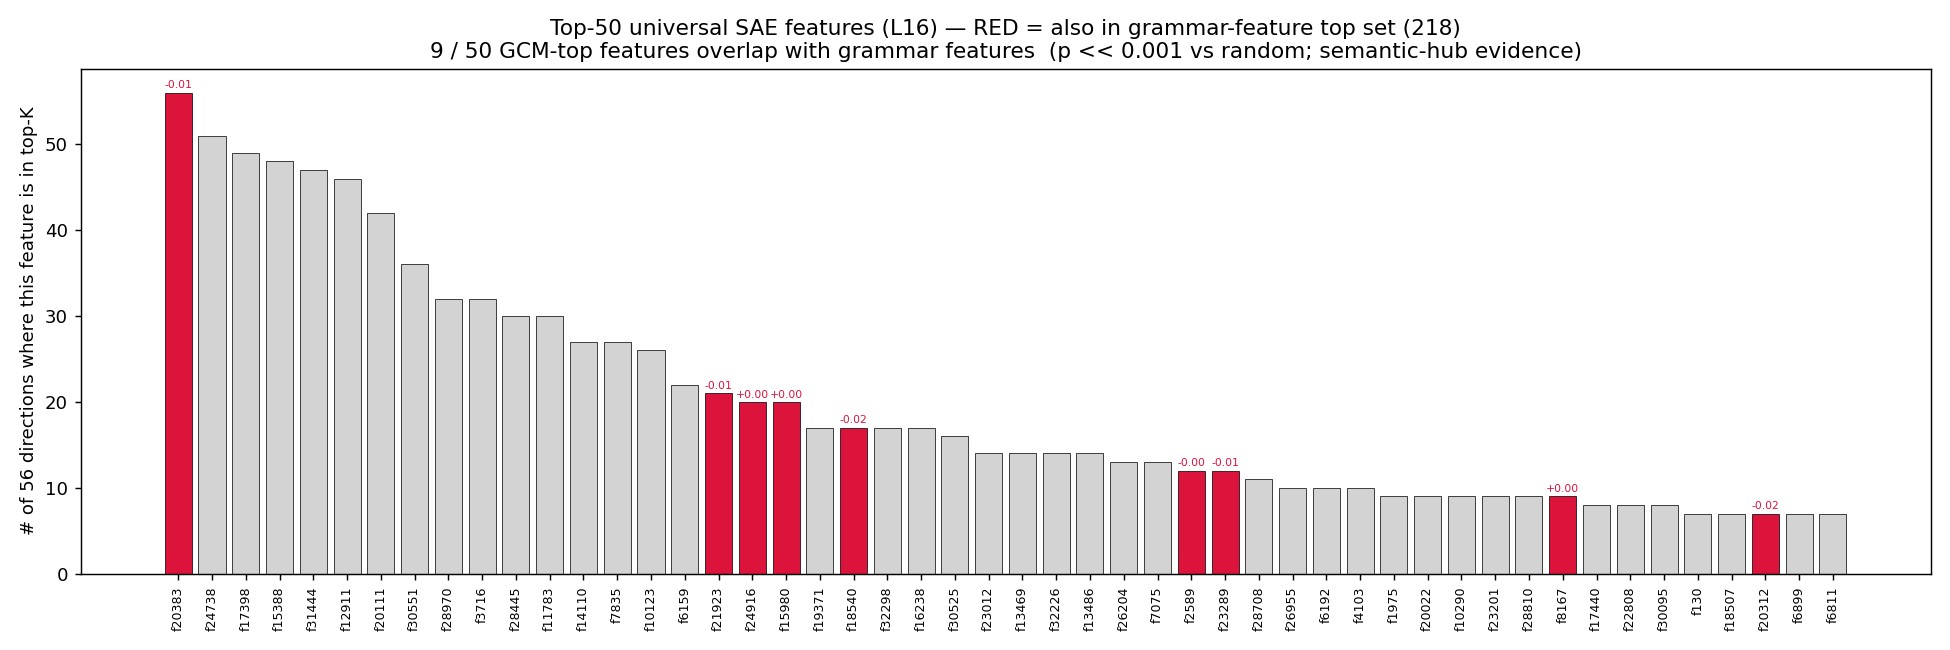
\includegraphics[width=\linewidth]{figures/meeting_sae_grammar_overlap.png}
\caption{These are the $50$ most direction-universal layer-16 SAE features, by number of the $56$ directions in which each appears in the top-$20$. Red bars mark features that also belong to the grammatical concepts feature set identified in an earlier experiment. As opposed to the $0.33$ expected by chance if the two sets were independent, $9/50$ overlap.}
\jb{TODO: verify the calculation needed to get 0.33}
\label{fig:gcm-grammar}
\end{figure}

\section{Finetuning on monolingual data is competitive with finetuning on parallel corpora}

\am{TODO @Jannik: prose + figures}

\section{Discussion and Conclusions}
We have found that a linear model conditioned on proxies for monolingual competence is a strong predictor of translation performance, that many components are influential in both translation and monolingual tasks, and that continued pre-trainining on monolingual data often yields similar gains in performance to continued pre-training with multilingual data. Together, these act as convergent evidence in support of our main hypothesis.

We emphasize that mechanisms selective for the translation task are still likely to exist; indeed, \am{TODO: Todd FV citation} find that there are components selective for word translation. It is likely that LLMs use a mixture of mechanisms \am{TODO: cite mixture of mechanisms paper} to achieve their translation performance. Our goal was to explain why monolingual pretraining is helpful for translation at all, and not to explain the entirety of LLM translation performance.

\section*{Limitations}

% Entries for the entire Anthology, followed by custom entries
\bibliography{custom}

\appendix

\section{Example Appendix}
\label{sec:appendix}

\begin{figure}[h]
\centering
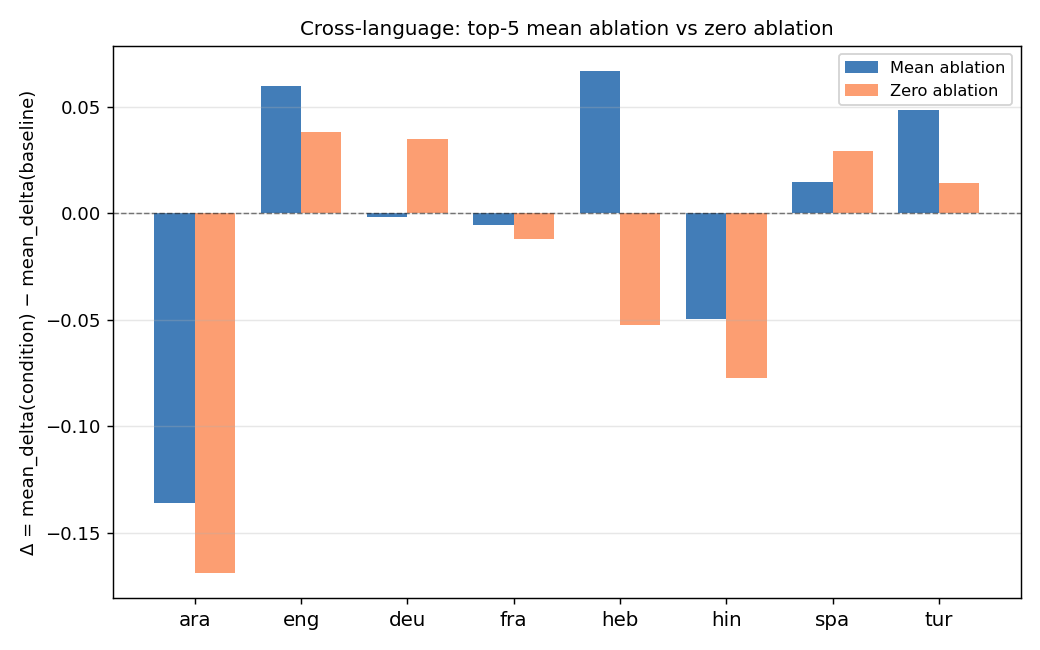
\includegraphics[width=\linewidth]{figures/cross_lang_mean_vs_zero.png}
\caption{Mean vs. zero ablation}
\end{figure}

\begin{figure}[h]
\centering
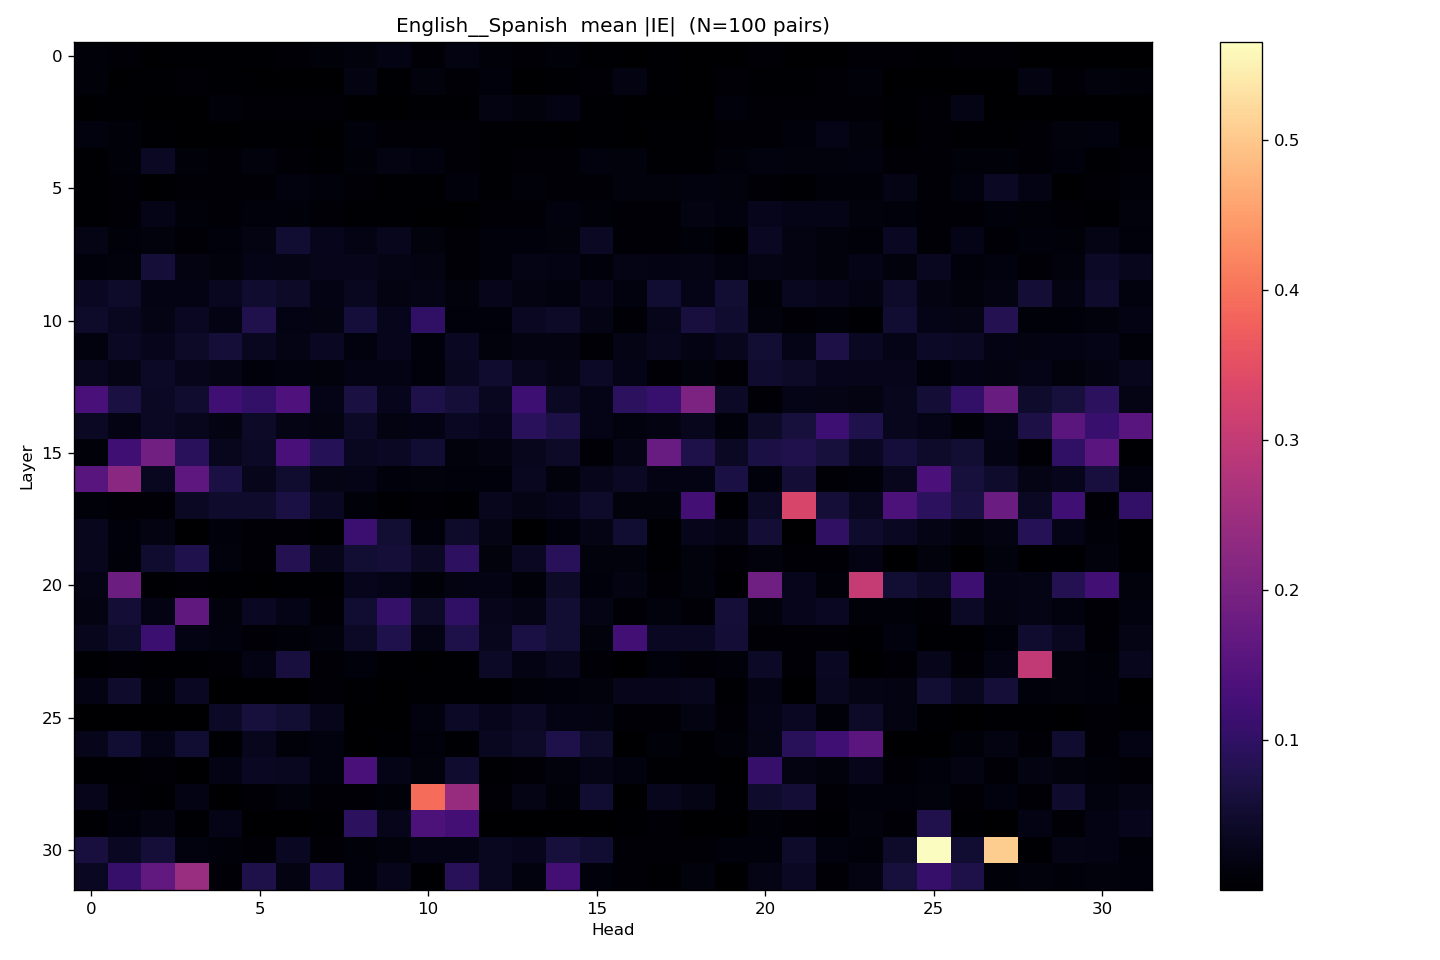
\includegraphics[width=.49\linewidth]{figures/English__Spanish_heads_heatmap.png}
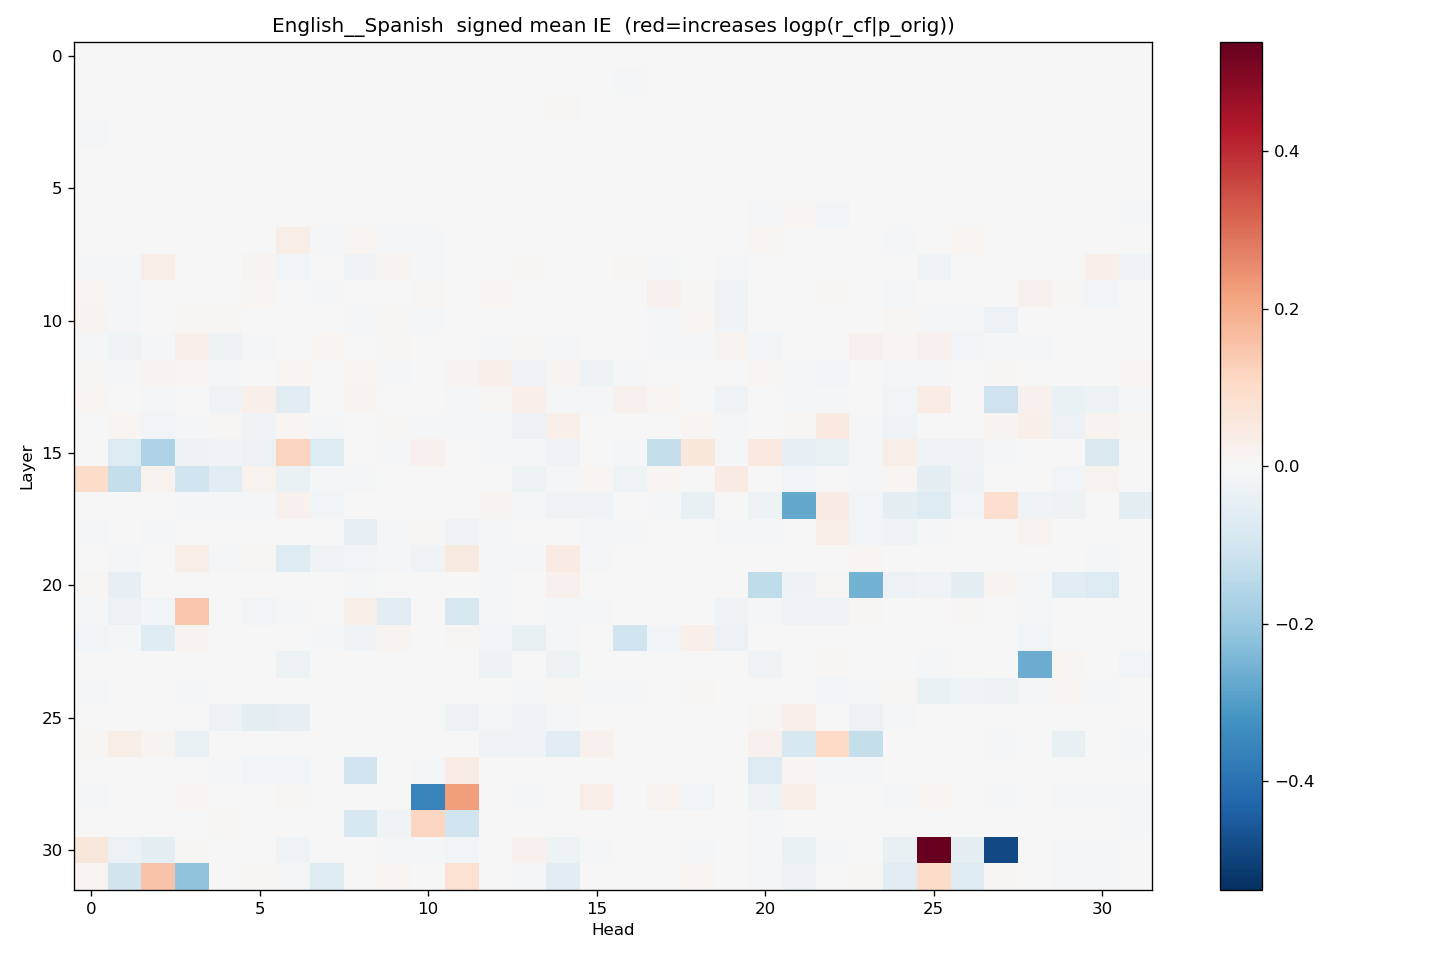
\includegraphics[width=.49\linewidth]{figures/English__Spanish_heads_signed_heatmap.png}
\caption{English$\to$Spanish GCM}
\end{figure}

\end{document}
